% \chapter{Brief Overview}
% % \label{ch:con}
% \section{Raw Data Source}

% \begin{figure}[ht]
%     \centering
%     \href{https://sentinels.copernicus.eu/documents/247904/4180891/Sentinel-2-infographic.pdf}{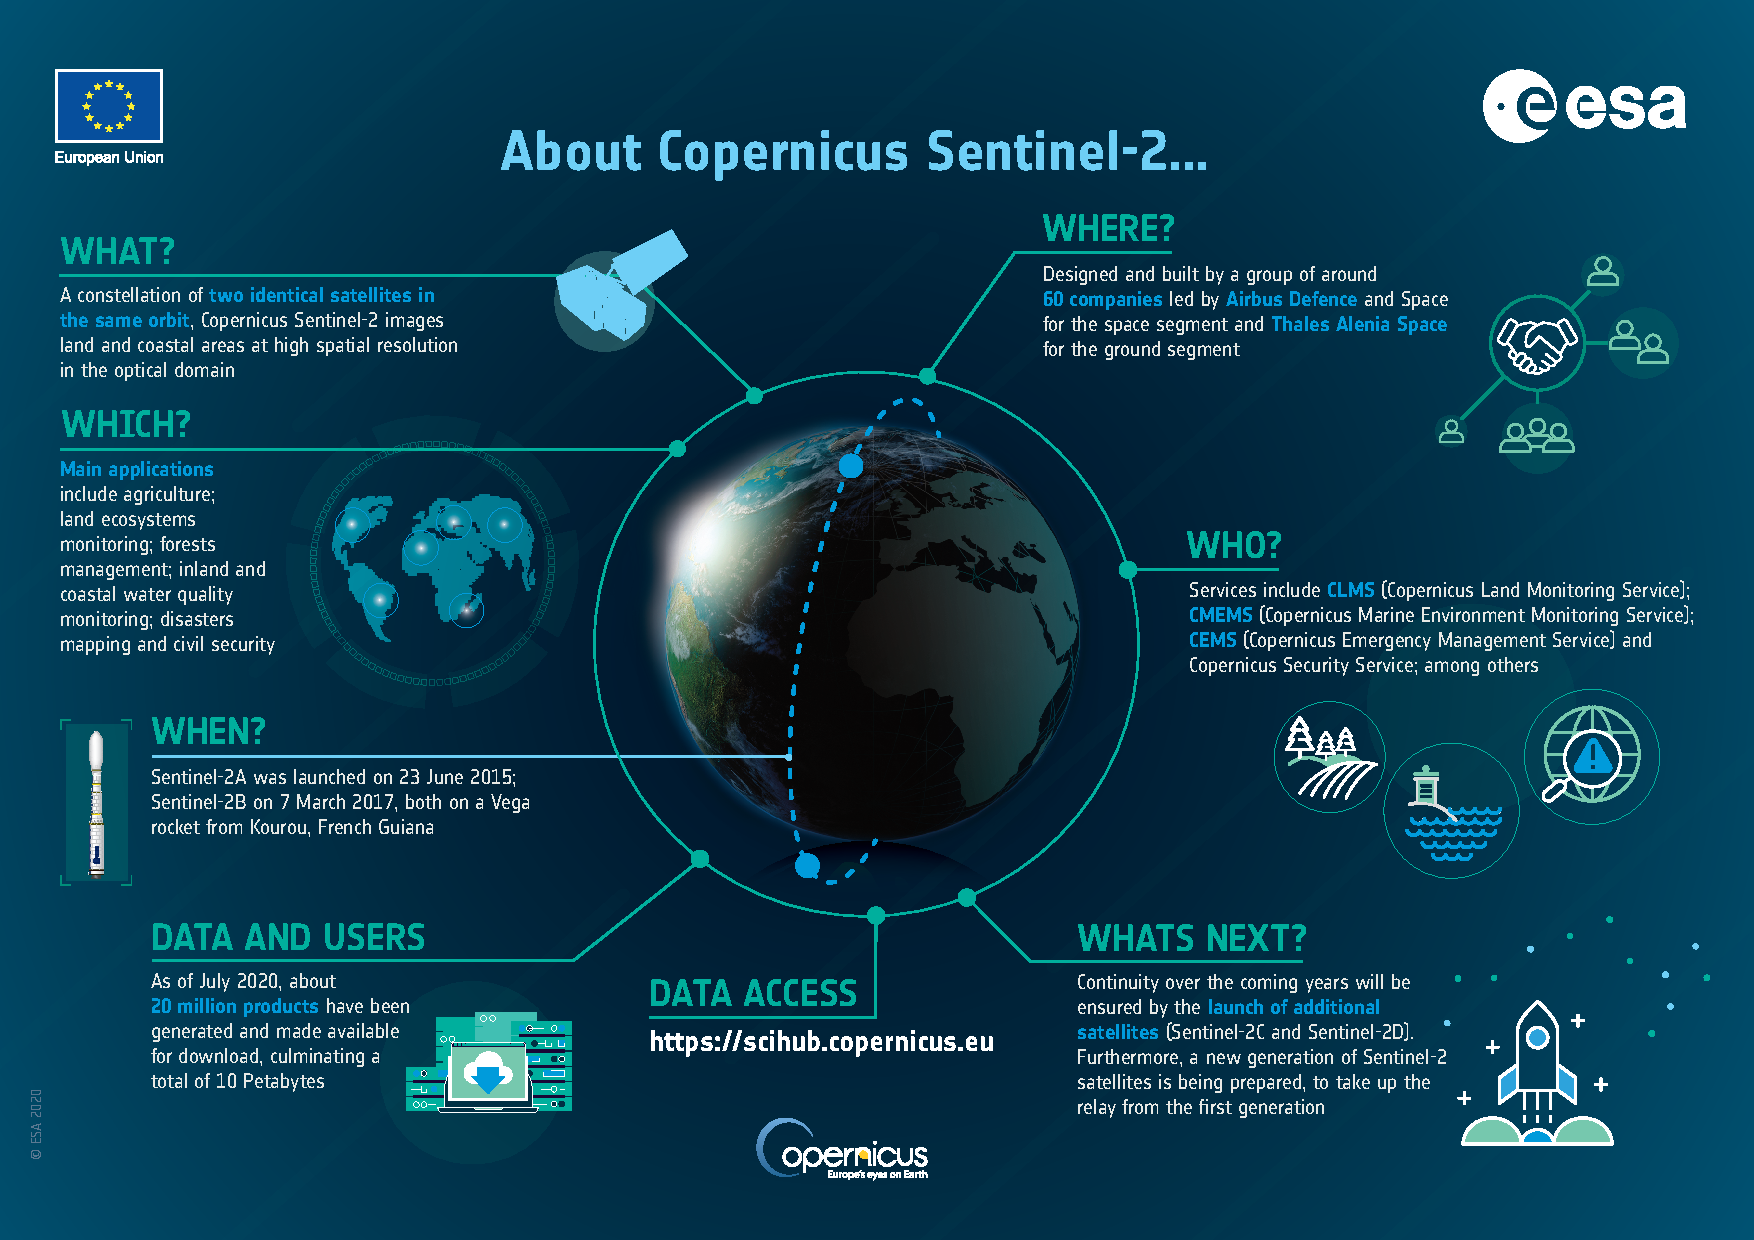
\includegraphics[width=0.9\linewidth]{figures_misc/Sentinel-2-infographic.pdf}}
%     \caption{A special infographic on the Sentinel- 2 mission was produced. It highlights important facts and achievements of the mission lifetime. Courtesy of \href{https://sentinels.copernicus.eu/web/sentinel/missions/sentinel-2}{ESA}.}
%     \label{fig:sentinel2_info}
% \end{figure}

% Fig.\,\ref{fig:sentinel2_info}, the Copernicus Sentinel-2 mission.
% Sentinel-2 is currently composed of two satellites, 2A and 2B, with future plans for 2C and 2D.
% Each has a revisit frequency of 10 days.
% The combined constellation has a revisit frequency of 5 days. 

% \begin{lstlisting}[language=Python, caption={Python code example for extracting and visualising Sentinel-2 data.}, label={code:gee_sentinel2_example}]
% def mask_s2_clouds(image):
%   """Masks clouds in a Sentinel-2 image using the QA band.

%   Args:
%       image (ee.Image): A Sentinel-2 image.

%   Returns:
%       ee.Image: A cloud-masked Sentinel-2 image.
%   """
%   # Select quality assessment at a 60 meter resolution.
%   qa = image.select('QA60')

%   # Bits 10 and 11 are clouds and cirrus, respectively.
%   cloud_bit_mask = 1 << 10
%   cirrus_bit_mask = 1 << 11

%   # Both flags should be set to zero, indicating clear conditions.
%   mask = (
%       qa.bitwiseAnd(cloud_bit_mask)
%       .eq(0)
%       .And(qa.bitwiseAnd(cirrus_bit_mask).eq(0))
%   )

%   return image.updateMask(mask).divide(10000)


% dataset = (
%     ee.ImageCollection('COPERNICUS/S2_SR_HARMONIZED')
%     .filterDate('2020-01-01', '2020-01-30')
%     # Pre-filter to get less cloudy granules.
%     .filter(ee.Filter.lt('CLOUDY_PIXEL_PERCENTAGE', 20))
%     .map(mask_s2_clouds)
% )

% visualization = {
%     'min': 0.0,
%     'max': 0.3,
%     'bands': ['B4', 'B3', 'B2'],
% }

% m = geemap.Map()
% m.set_center(83.277, 17.7009, 12)
% m.add_layer(dataset.mean(), visualization, 'RGB')
% m
% \end{lstlisting}

% Data to be extracted using Google Earth Engine through its \href{https://developers.google.com/earth-engine/apidocs}{Python API} such as the \href{https://developers.google.com/earth-engine/datasets/catalog/COPERNICUS_S2_SR_HARMONIZED#colab-python}{example} in Listing\,\ref{code:gee_sentinel2_example}. If the environment is set-up correctly, this code displays an interactive map overlaid with Sentinel-2 temporal mean values of the red, green, and blue (RGB) bands. Smaller sample images were extracted and are shown in Fig.\,\ref{fig:sample_100_pixelside} and Fig.\,\ref{fig:sample_1000_pixelside}.

% \begin{figure}[ht]
%     \centering
%     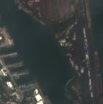
\includegraphics[width=0.9\linewidth]{figures_sentinel/sample_100_pixelside.png}
%     \caption{A 100 by 100 pixel (1\,km$^2$) RGB extract from Sentinel-2.}
%     \label{fig:sample_100_pixelside}
% \end{figure}

% \begin{figure}[ht]
%     \centering
%     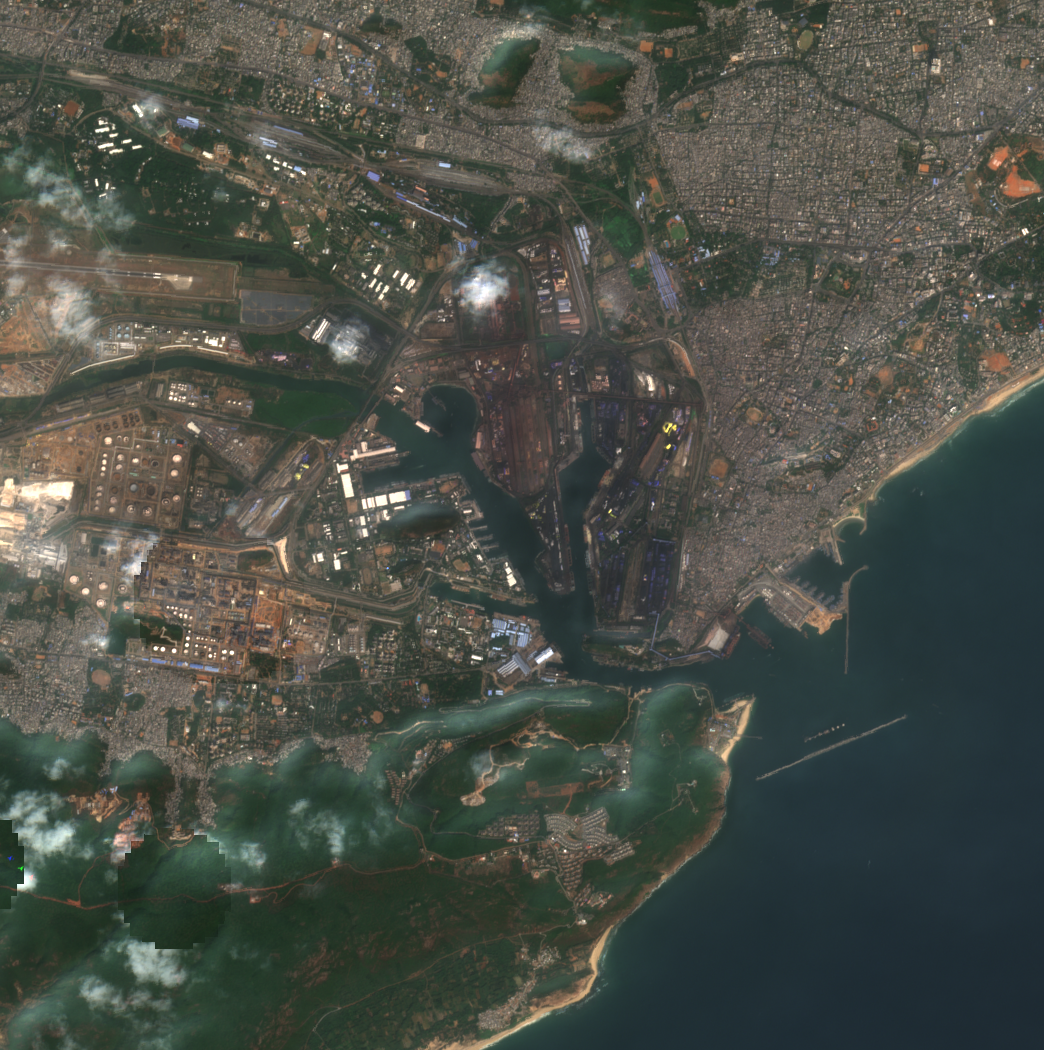
\includegraphics[width=0.9\linewidth]{figures_sentinel/sample_1000_pixelside.png}
%     \caption{A 1000 by 1000 pixel (100\,km$^2$) RGB extract from Sentinel-2.}
%     \label{fig:sample_1000_pixelside}
% \end{figure}

% \section{Training Data}

% Most used seems to be forest inventory data.
% Could not find much from UK Forestry.

% \section{ML Estimators}

% Estimators mainly in use appear to be SVM and RF. Both appear to be usable directly within the Earth Engine Python API. 

% \subsection{Support Vector Machines (SVM)}

% SVM works by mapping data to a high-dimensional feature space so that data points 
% can be categorized, even when the data are not otherwise linearly separable.

% \subsection{Random Forest (RF)}

% Combines the output of multiple decision trees to reach a single result. A decision tree is a decision support hierarchical model that uses a tree-like model of decisions and their possible consequences, including chance event outcomes, resource costs, and utility.


% \section{Why Classify Trees}

% \begin{itemize}
%     \item Broadleaved species – such as oak, beech and maple – are best because they have a larger surface area of leaves which generates more photosynthesis, whereas conifers absorb more heat. \hyperlink{https://www.glendale-services.co.uk/latest-news/plant-the-right-trees-to-combat-climate-change/}{Source.}
%     \item 
% \end{itemize}

% \section{Tentative Literature Review}

% \begin{table}[h!]
%     \centering
%     \caption{Sentinel-2 tree species classification literature summary.}
%     \label{tab:_ex_tab}
%     \begin{tabular}{lllll}     
%         \toprule
%         % \multicolumn{2}{c}{Bike} \\
%         % \cmidrule(r){1-2}
%         Literature             & Location          & Estimators   & Trees                    & S2 Bands \\
%         \midrule
%         \cite{germany_bavaria} & Bavaria, GER      & SVM, RF      & \makecell[l]{broad-leaved,\\ coniferous} & 8, 2, 3 \\
%         \cite{china_northeast} & Northeast China   & SVM, RF, NNs & & \\
%         \cite{copernicus_main} & Lower Saxony, GER & NNs          & \makecell[l]{pine, beech, spruce,\\ oak, others} & \\
%         \bottomrule
%     \end{tabular}
% \end{table}

% \section{Questions}

% \begin{itemize}
%     \item Surface Reflectance vs Top-of-Atmosphere Reflectance
%     \item Transferability of local models
%     \item Further data, e.g. NASA's \href{http://wiki.gis.com/wiki/index.php/Digital_Elevation_Model}{Digital Elevation Model}
% \end{itemize}
